\chapter{Практические результаты}
\section{Параметры компьютера, производящего вычисления}
Все вычисления были выполнены на ноутбуке Acer с процессором \textbf{Intel(R) Core(TM) i7-4710HQ CPU @ 2.50GHz} под операционной системой \textbf{Ubuntu 16.04 LTS}.

Реализации всех алгоритмов были написаны на языке C++, и были скомпилированы с флагами \textbf{-std=c++14 -O2} используя компилятор \textbf{g++ (Ubuntu 5.4.0-6ubuntu1~16.04.4) 5.4.0 20160609}.

\section{Наибольшая общая Абелева подстрока}
\subsection{Случай бинарного алфавита}

Первое, что мы сделаем~--- посмотрим, как себя ведет на практике матожидание наибольшей общей Абелевой подстроки двух случайных бинарных строк. 

Мы выполнили $10^4$ запусков поиска НОАП для различных значений $n$ до $10^4$. Такого количества запусков оказалось вполне достаточно, чтобы среднее значение НОАП стабилизировалось. Полученный результат можно увидеть на рисунке 2.

\begin{figure}[h]
\center{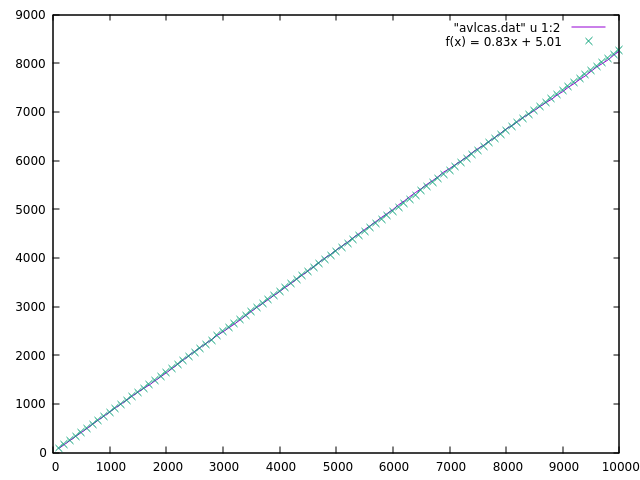
\includegraphics[scale=1]{pics/avlcas.png}}
\caption{зависимость матожидания НОАП от длин строк}
\end{figure}

Видно, что функция ведет себя практически как прямая $y=0.83x$, что подтверждает полученные теоретические линейные оценки как сверху, так и снизу.

%\subsection{Общий случай}
%Пусто? Ну я канеш могу закодить то что я придумал но не оч хочется(((

\subsection{Случай большого алфавита}

Будем сравнивать время работы предложенного в этой статье алгоритма за $\mathcal{O}(n^2 \log \sigma)$ с алгоритмом, предложенным A. Attabi et al \cite{1}. Главными достоинствами этого алгоритма является необычайная простота, котороая приводит к очень маленькой константе, скрытой во временной оценке, потому что в нем не используется никаких тяжелых алгоритмов. Алгоритм S. Grabowski et al \cite{4} за $\mathcal{O}
(n^2 \log \sigma)$ имеет такую же временную асимптотику, поэтому с ним сравнение не проводилось: есть все основания полагать, что он работает в несколько (как минимум, в два) раз медленнее из-за эвристик, приводящих к уменьшению потребления памяти.

Так же в процессе анализа было принято решение не сравнивать с алгоритмом S. Grabowski et al \cite{4} за $\mathcal{O}(n^2 \log^2 n \log^* n)$, потому что в процессе ознакомления с ним было выяснено, что у него слишком большая скрытая константа~--- алгоритм получен в результате деамортизации недетерминированного, используя для этого довольно ресурсоемкие операции и структуры данных.

В свою очередь, алгоритм, предложенный в настоящей работе, достаточно тяжелый как в плане написания кода, так и имеет сложно оцениваемую скрытую константу времени работы из-за необходимости в аккуратной работе с памятью. Представляет большой интерес понимание того, является ли данный алгоритм лишь теоретическим улучшением существующих, или все же он дает ощутимое ускорение на практике.

Сравнение времени работы предложенного алгоритма в зависимости от $n$ на тесте из двух строк длины $n$, состоящих из случайных символов из алфавита мощности $n$, представлено на рисунке 3.

\begin{figure}[h]
\center{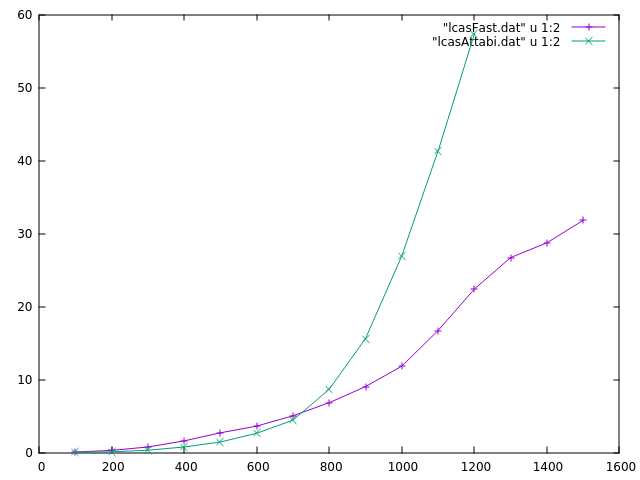
\includegraphics[scale=1]{pics/common_lcas_n.png}}
\caption{Зависимость времени работы алгоритмов от $n$ на случайной строке над большим алфавитом}
\end{figure}

Таким образом, можно с уверенностью сказать, что начиная с не очень большого $n$ предложенный алгоритм начинает выигрывать у стандартной реализации известного алгоритма, и этот выигрыш будет только увеличиваться из-за более хорошей асимптотики.

К сожалению, несмотря на строго более хорошую асимптотику, на маленьких тестовых данных предложенный алгоритм работает несколько медленнее, чем алгоритм из \cite{1}. Это можно объяснить наличием скрытой в асимптотике алгоритма константой, но она достаточно мала, чтобы все равно обеспечить выигрыш на реальных данных.

\section{Количество Абелевых подквадратов}

Мы реализовали алгоритм нахождения числа Абелевых подквадратов с помощью сведения к алгоритму решения монотонного ограниченного случая $3SUM^+$. Он был протестирован на строках из одинаковых символов, и на наборе пар случайных бинарных строк. Как оказалось, константа алгоритма довольно велика, и на практике он показал себя достаточно плохо, в несколько раз проигрывая наивному решению за $\mathcal{O}(n^2)$.

\begin{figure}[h]
\center{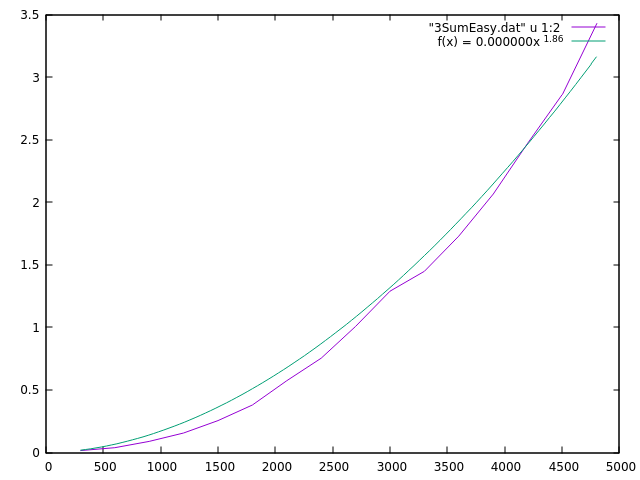
\includegraphics[scale=1]{pics/4.png}}
\caption{зависимость средней времени работы на строке из одинаковых символов от ее длины}
\end{figure}

На рисунке 4 можно увидеть зависимость времени работы решения в секундах от $n$ на тесте из строки, состоящей из $n$ одинаковых символов. График действительно довольно похож на $\mathcal{O}(n^{1.86})$, но из-за нескольких логарифмов в асимптотике растет несколько быстрее. 

\begin{figure}[h]
\center{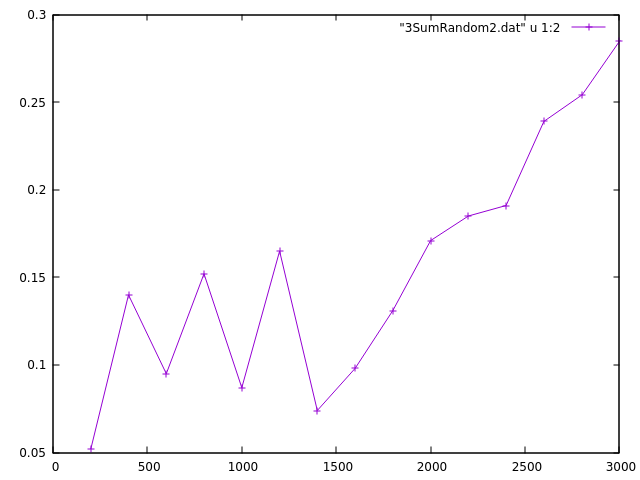
\includegraphics[scale=1]{pics/5.png}}
\caption{зависимость средней времени работы на случайной строке от ее длины}
\end{figure}

На рисунке 5 можно увидеть зависимость времени работы решения в секундах от $n$ на тесте из строки, состоящей из $n$ случайно сгенерированных символов.

Время работы алгоритма довольно сильно меняется как от запуска к запуску из-за разных тестов, так и от различных значений $n$, так как различные ветки программы выполняются с разными вероятностями и работают разное время~--- не приходится удивляться некоторому увеличению производительности при увеличении $n$.
